\chapter*{More figures}
\addcontentsline{toc}{chapter}{More figures}

Some figures are referred to in the text but not placed directly under the text. These are included in this list. All figures are high resolution thus zooming in the PDF should be viable to get a clearer view.

%------------------------------------

\section*{Overview of training set}

\begin{figure}[H]
    \begin{center}
        \fbox{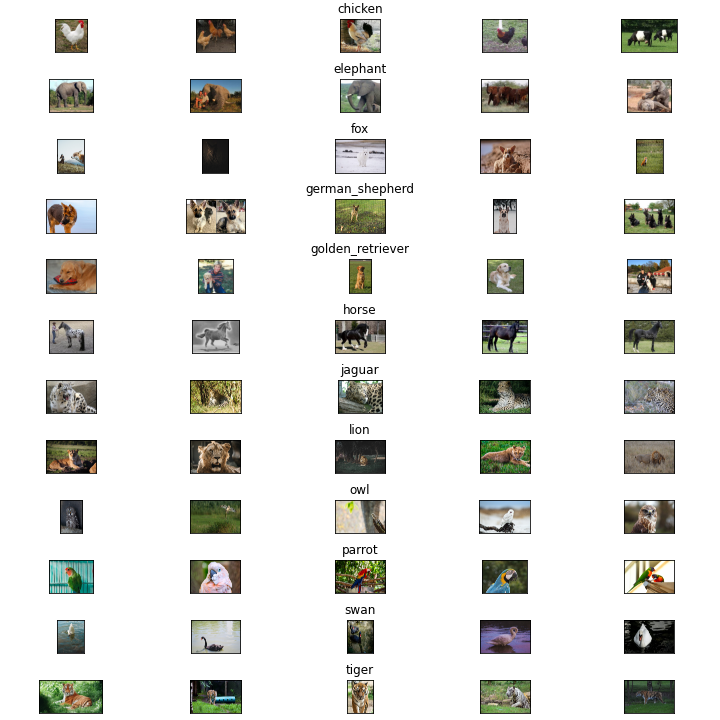
\includegraphics[width=0.70\linewidth]{images/1-data_analysis-labeled_data_overview.png}}
    \end{center}
    \captionsetup{width=0.65\linewidth}
    \captionsetup{justification=centering}
    \caption{An overview of the supplied data per class.}
    \label{fig:1-data_analysis-labeled_data_overview.png}
\end{figure}

%------------------------------------

\section*{Overview of features data}

\begin{figure}[H]
    \fbox{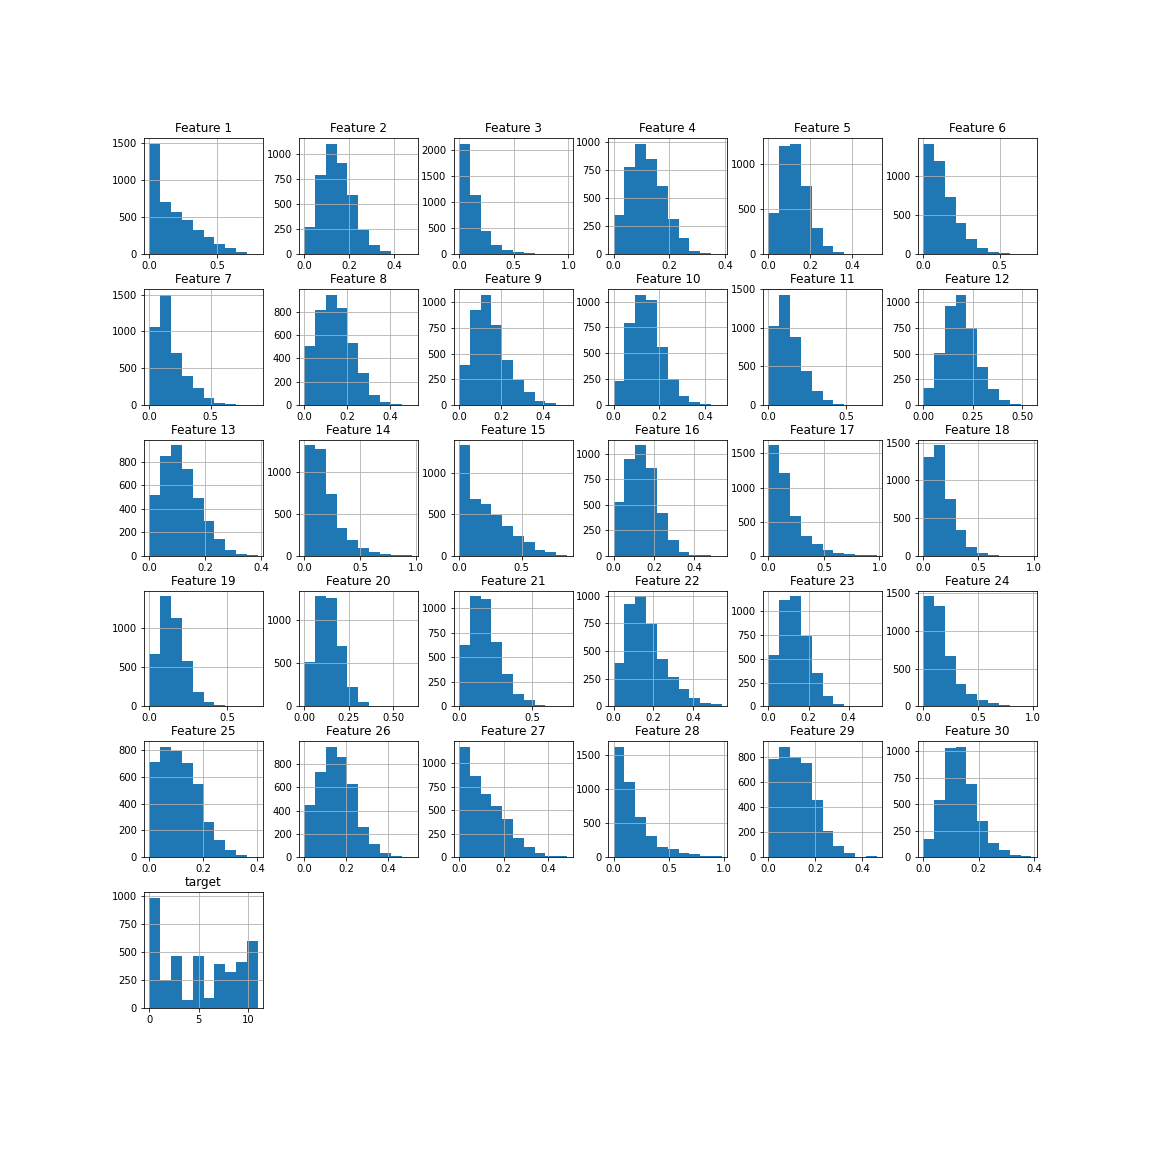
\includegraphics[width=1\linewidth]{images/1-data_analysis-feature_representation.png}}
    \captionsetup{width=0.85\linewidth}
    \captionsetup{justification=centering}
    \caption{An overview of the first 30 features data from a SIFT descriptor.}
    \label{fig:1-data_analysis-feature_representation}
\end{figure}

%------------------------------------

\section*{Linear baseline model - input optimisation (small)}

\begin{figure}[H]
  \centering
  \begin{minipage}[b]{0.4\textwidth}
    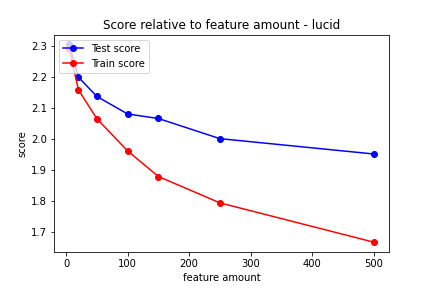
\includegraphics[width=\textwidth]{images/2-LBM-feature_amount_lucid_small_values.png}
  \end{minipage}
  \hfill
  \begin{minipage}[b]{0.4\textwidth}
    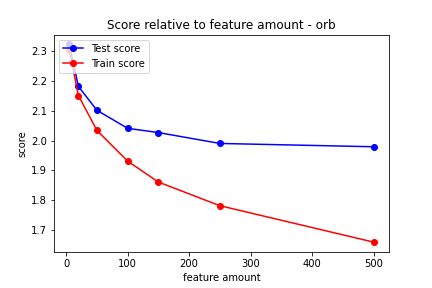
\includegraphics[width=\textwidth]{images/2-LBM-feature_amount_orb_small_values.png}
  \end{minipage}
\end{figure}

\begin{figure}[H]
  \centering
  \begin{minipage}[b]{0.4\textwidth}
    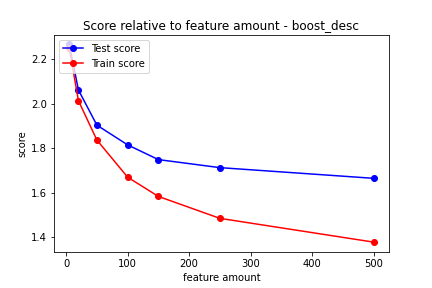
\includegraphics[width=\textwidth]{images/2-LBM-feature_amount_boost_desc_small_values.png}
  \end{minipage}
  \hfill
  \begin{minipage}[b]{0.4\textwidth}
    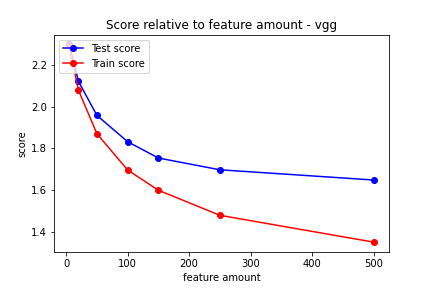
\includegraphics[width=\textwidth]{images/2-LBM-feature_amount_vgg_small_values.png}
  \end{minipage}
\end{figure}

\begin{figure}[H]
  \centering
  \begin{minipage}[b]{0.4\textwidth}
    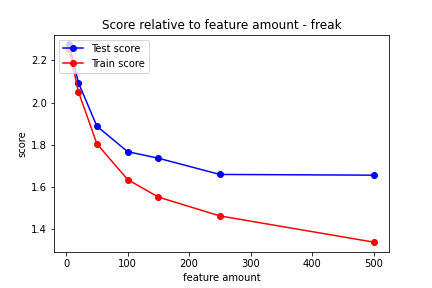
\includegraphics[width=\textwidth]{images/2-LBM-feature_amount_freak_small_values.png}
  \end{minipage}
  \hfill
  \begin{minipage}[b]{0.4\textwidth}
    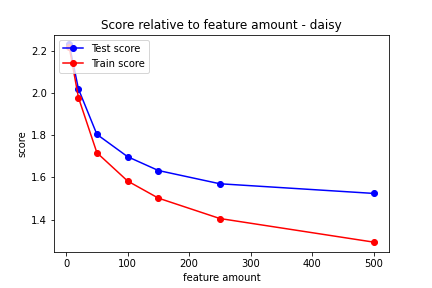
\includegraphics[width=\textwidth]{images/2-LBM-feature_amount_daisy_small_values.png}
  \end{minipage}
\end{figure}

\begin{figure}[H]
  \centering
  \begin{minipage}[b]{0.4\textwidth}
    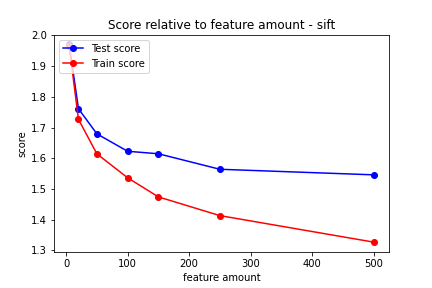
\includegraphics[width=\textwidth]{images/2-LBM-feature_amount_sift_small_values.png}
  \end{minipage}
\end{figure}

%------------------------------------

\section*{Linear baseline model - input optimisation (large)}

\begin{figure}[H]
  \centering
  \begin{minipage}[b]{0.4\textwidth}
    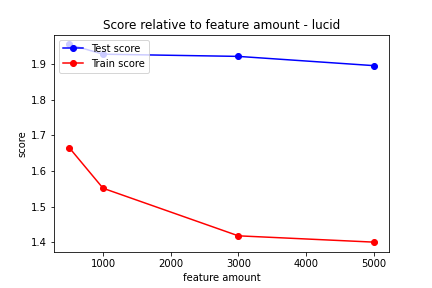
\includegraphics[width=\textwidth]{images/2-LBM-feature_amount_lucid_large_values.png}
  \end{minipage}
  \hfill
  \begin{minipage}[b]{0.4\textwidth}
    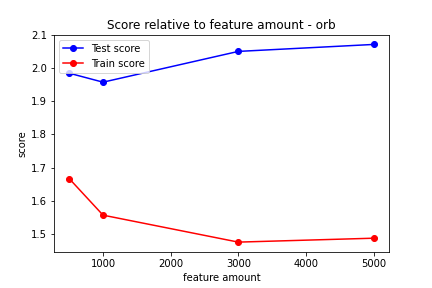
\includegraphics[width=\textwidth]{images/2-LBM-feature_amount_orb_large_values.png}
  \end{minipage}
\end{figure}

\begin{figure}[H]
  \centering
  \begin{minipage}[b]{0.4\textwidth}
    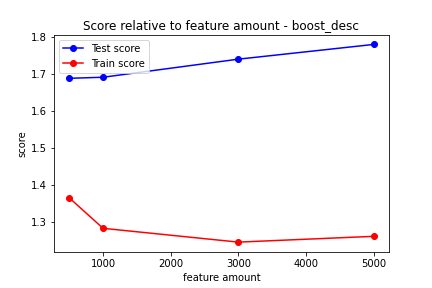
\includegraphics[width=\textwidth]{images/2-LBM-feature_amount_boost_desc_large_values.png}
  \end{minipage}
  \hfill
  \begin{minipage}[b]{0.4\textwidth}
    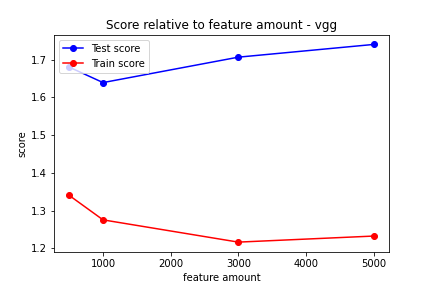
\includegraphics[width=\textwidth]{images/2-LBM-feature_amount_vgg_large_values.png}
  \end{minipage}
\end{figure}

\begin{figure}[H]
  \centering
  \begin{minipage}[b]{0.4\textwidth}
    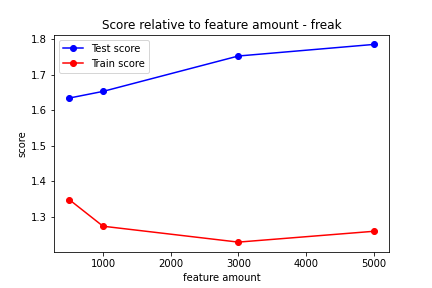
\includegraphics[width=\textwidth]{images/2-LBM-feature_amount_freak_large_values.png}
  \end{minipage}
  \hfill
  \begin{minipage}[b]{0.4\textwidth}
    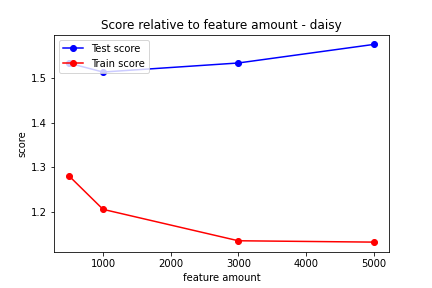
\includegraphics[width=\textwidth]{images/2-LBM-feature_amount_daisy_large_values.png}
  \end{minipage}
\end{figure}

\begin{figure}[H]
  \centering
  \begin{minipage}[b]{0.4\textwidth}
    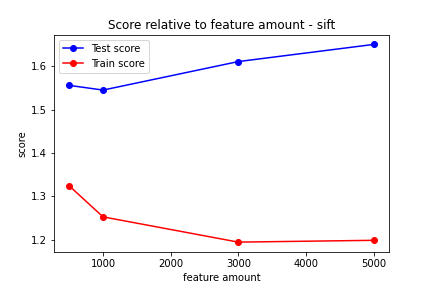
\includegraphics[width=\textwidth]{images/2-LBM-feature_amount_sift_large_values.png}
  \end{minipage}
\end{figure}

%------------------------------------

\section*{Linear baseline model - optimal DAISY}

\begin{figure}[H]
    \fbox{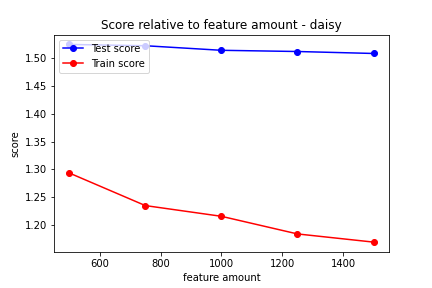
\includegraphics[width=1\linewidth]{images/2-LBM-feature_amount_daisy_daisy_optimal.png}}
    \captionsetup{width=0.85\linewidth}
    \captionsetup{justification=centering}
    \caption{An extra test for finding the optimal feature amounts for the DAISY descriptor.}
    \label{fig:2-LBM-feature_amount_daisy_daisy_optimal}
\end{figure}

%------------------------------------

\section*{Linear baseline model - class weight parameter}

\begin{figure}[H]
    \fbox{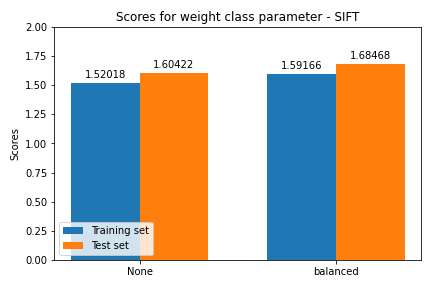
\includegraphics[width=1\linewidth]{images/2-LBM-model_weight_class.png}}
    \captionsetup{width=0.85\linewidth}
    \captionsetup{justification=centering}
    \caption{Average multi-class Log Loss score over 10 iterations.}
    \label{fig:2-LBM-model_weight_class}
\end{figure}

%------------------------------------

\section*{Linear baseline model - fit intercept parameter}

\begin{figure}[H]
    \fbox{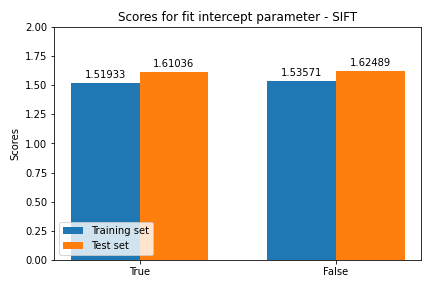
\includegraphics[width=1\linewidth]{images/2-LBM-model_fit_intercept.png}}
    \captionsetup{width=0.85\linewidth}
    \captionsetup{justification=centering}
    \caption{Average multi-class Log Loss score over 5 iterations.}
    \label{fig:2-LBM-model_fit_intercept}
\end{figure}